\documentclass{article}
\usepackage{pgfplots}
\usepackage[top=2cm,left=2cm,right=2cm,bottom=2cm]{geometry}
\pgfplotsset{compat=1.17}


\begin{document}
\begin{center}
    \huge Calculus III Homework 3 Question 3\\
    Section 10.2 \# 9 - 12\\
\end{center}
\vspace{50pt}
9. Find the sum of $<-1,4>$ and $<6,-2>$ and graph them\\
\begin{center}
  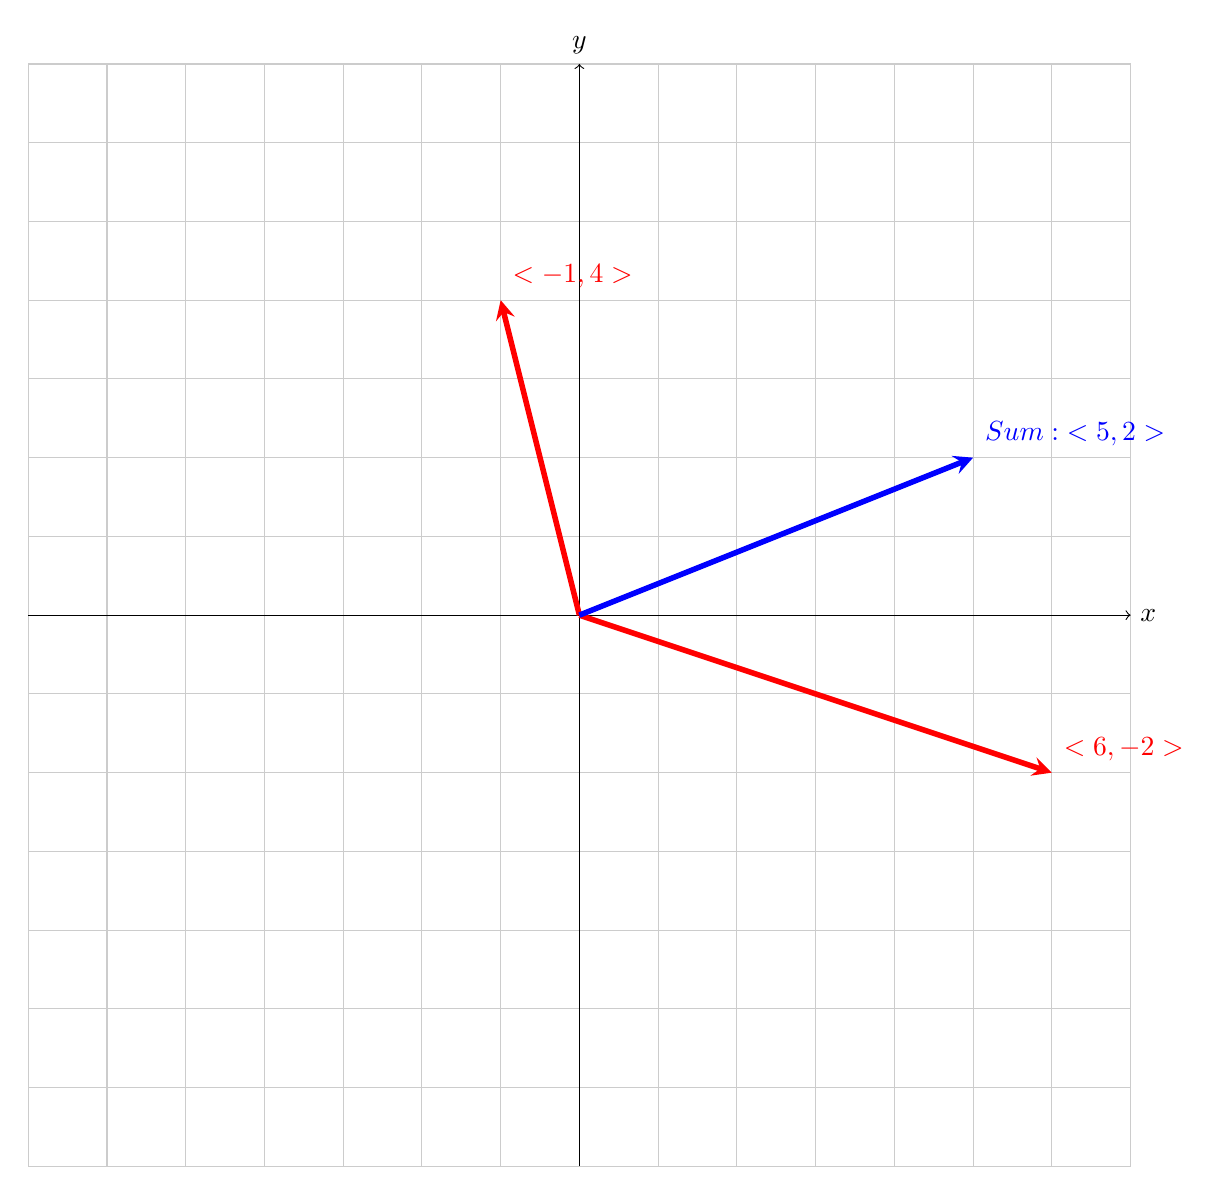
\begin{tikzpicture}
  \draw[thin,gray!40] (-7,-7) grid (7,7);
  \draw[->] (-7,0)--(7,0) node[right]{$x$};
  \draw[->] (0,-7)--(0,7) node[above]{$y$};
  \draw[line width=2pt,red,-stealth](0,0)--(-1,4) node[anchor=south west]{${<-1,4>}$};
  \draw[line width=2pt,red,-stealth](0,0)--(6,-2) node[anchor=south west]{${<6,-2>}$};
  \draw[line width=2pt,blue,-stealth](0,0)--(5,2) node[anchor=south west]{$Sum: {<5,2>}$};
\end{tikzpicture}
\end{center}

\newpage
10. Find the sum of $<3,-1>$ and $<-1,5>$ and graph them\\
\begin{center}
  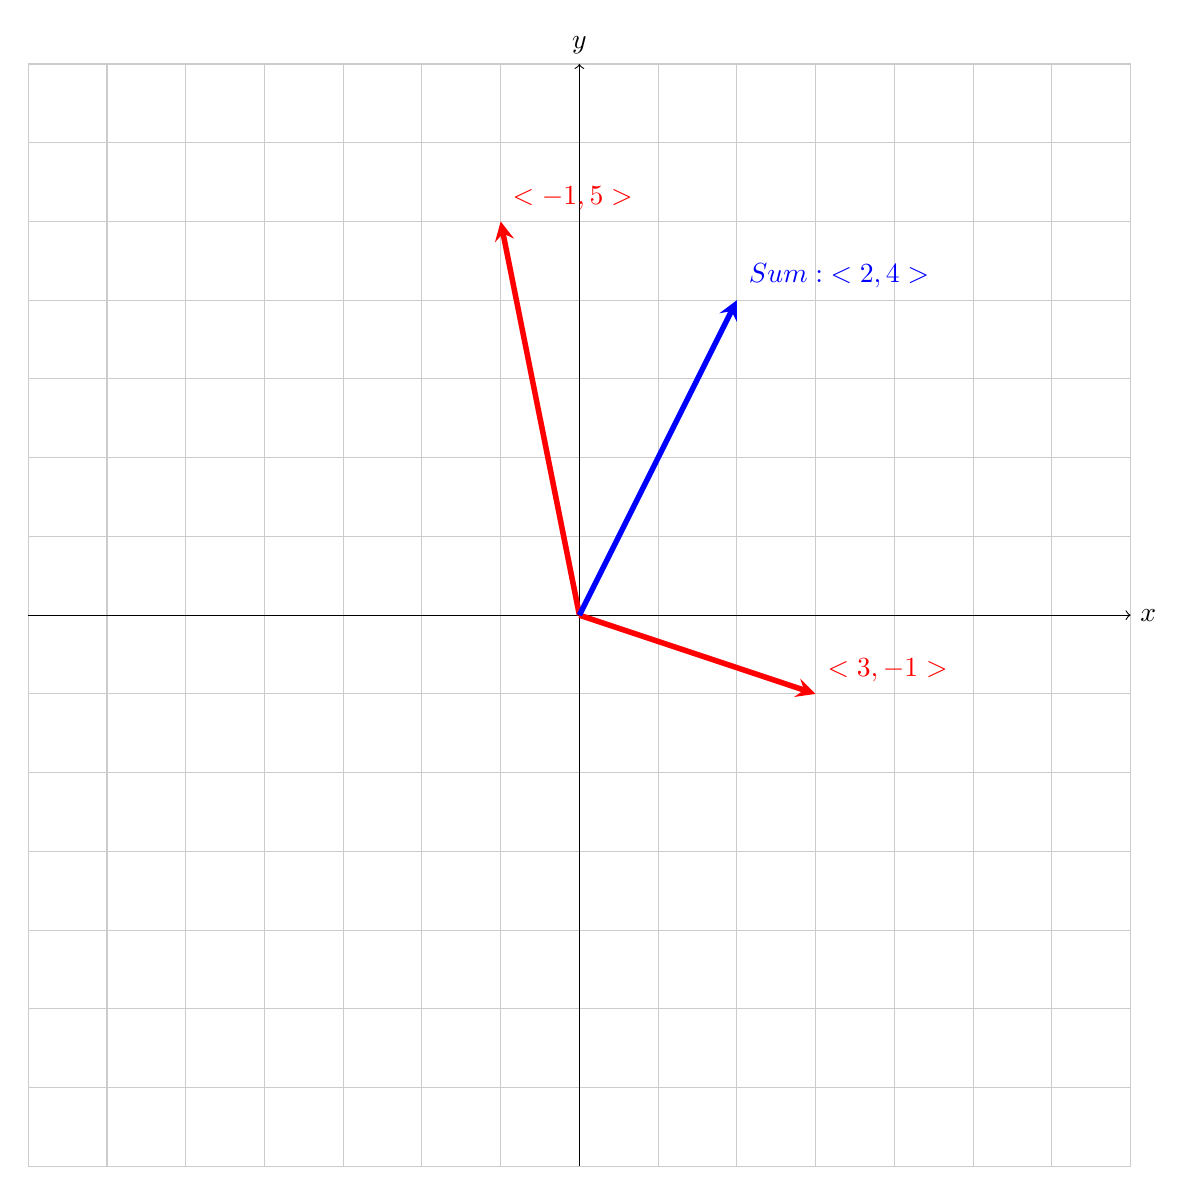
\begin{tikzpicture}
  \draw[thin,gray!40] (-7,-7) grid (7,7);
  \draw[->] (-7,0)--(7,0) node[right]{$x$};
  \draw[->] (0,-7)--(0,7) node[above]{$y$};
  \draw[line width=2pt,red,-stealth](0,0)--(3,-1) node[anchor=south west]{${<3,-1>}$};
  \draw[line width=2pt,red,-stealth](0,0)--(-1,5) node[anchor=south west]{${<-1,5>}$};
  \draw[line width=2pt,blue,-stealth](0,0)--(2,4) node[anchor=south west]{$Sum: {<2,4>}$};
\end{tikzpicture}
\end{center}

\newpage
11. Find the sum of $<3,0,1>$ and $<0,8,0>$ and graph them\\
\begin{center}
  \begin{tikzpicture}
  % \draw[thin,gray!40] (-9,-9) grid (9,9);
  \draw[->] (-9,0,0)--(9,0,0) node[right]{$x$};
  \draw[->] (0,-9,0)--(0,9,0) node[above]{$y$};
  \draw[->] (0,0,-9)--(0,0,9) node[above]{$z$};
  \draw[line width=2pt,red,-stealth](0,0,0)--(3,0,1) node[anchor=south west]{${<3,0,1>}$};
  \draw[line width=2pt,red,-stealth](0,0,0)--(0,8,0) node[anchor=south west]{${<0,8,0>}$};
  \draw[line width=2pt,blue,-stealth](0,0,0)--(3,8,1) node[anchor=south west]{$Sum: {<3,8,1>}$};
\end{tikzpicture}
\end{center}

\newpage
12. Find the sum of $<1,3,-2>$ and $<1,3,4>$ and graph them\\
\begin{center}
  \begin{tikzpicture}
  % \draw[thin,gray!40] (-7,-7) grid (7,7);
  \draw[->] (-7,0,0)--(7,0,0) node[right]{$x$};
  \draw[->] (0,-7,0)--(0,7,0) node[above]{$y$};
  \draw[->] (0,0,-7)--(0,0,7) node[above]{$z$};
  \draw[line width=2pt,red,-stealth](0,0,0)--(1,3,-2) node[anchor=south west]{${<1,3,-2>}$};
  \draw[line width=2pt,red,-stealth](0,0,0)--(0,0,6) node[anchor=south west]{${<0,0,6>}$};
  \draw[line width=2pt,blue,-stealth](0,0,0)--(1,3,4) node[anchor=south west]{Sum: ${\langle1,3,4\rangle}$};
\end{tikzpicture}
\end{center}

\end{document}